%%%%%%%%%%%%%%%%%%%%%%%%%%%%%%%%%%%%%%%%%%%%%%
%%%%%%%%%%%%%%%%%%%%%%%%%%%%%%%%%%%%%%%%%%%%%%
%%% Master Thesis Template by Fabian Schär %%%
%%%%%%%%%%%%%%%%%%%%%%%%%%%%%%%%%%%%%%%%%%%%%%
%%%%%%%%%%%%%%%%%%%%%%%%%%%%%%%%%%%%%%%%%%%%%%

%%%%%%%%%%%%%%%%%%%%%%%%%%%%%%%%%%%%%%
%%% Packages and Document Settings %%%
%%%%%%%%%%%%%%%%%%%%%%%%%%%%%%%%%%%%%%

\documentclass[12pt,a4paper,titlepage,oneside,english]{article}

%%% Main Packages %%%
\usepackage[english]{babel}
%\usepackage[ngerman]{babel} % Use this option for German settings.
\usepackage[T1]{fontenc}
\usepackage[utf8]{inputenc}

%%% Additional Packages %%%
\usepackage{cite}
\usepackage{framed}
\usepackage{graphicx}
%\usepackage[german]{fancyref}
\usepackage[german,hidelinks]{hyperref} %hidelinks
\usepackage{multirow}
\usepackage[round]{natbib}
\usepackage{setspace}
\usepackage{geometry}
\usepackage{pst-all} % Not working with Sweave!!!
\usepackage{tikz}
\usetikzlibrary{positioning, intersections}

%%% Math Packages %%%
\usepackage{amsmath}
\usepackage{amstext}
\usepackage{amssymb}
\usepackage{theorem}
\usepackage{epsfig}
\usepackage{longtable}

%%% Layout Specifications %%%
\geometry{a4paper, top=35mm, left=40mm, right=40mm, bottom=45mm,
headsep=10mm, footskip=12mm}

%%% Parskip Settings %%%
\setlength{\parskip}{3mm}
\setlength{\parindent}{0mm}

%%% Document Specifications %%%
\title{Template Master's Thesis}
\author{John Doe}


%%%%%%%%%%%%%%%%%%
%%% Title Page %%%
%%%%%%%%%%%%%%%%%%

\begin{document}
%\begin{titlepage}
\begin{center}
\vspace{1em}
\large{Master Thesis}\\
\huge Developing Address Clustering Heuristics for Account-Based Blockchain Networks:\\ An Analysis based on a Specific Address Set \\
\Large \vspace{1em}
Dario Thürkauf
\end{center}

\vspace{1em}
\normalsize
\begin{flushleft}
Supervised by:\\ 
Prof. Dr. Fabian Schär \\ 
Professor for Distributed Ledger Technologies and Fintech \\
Center for Innovative Finance, University of Basel
\end{flushleft}

\vspace{1em}
\onehalfspacing
\begin{center}
\section*{Abstract}
\end{center}
Assentiar consuetae ha opinionum mentemque ob ii. Ne conflantur de intelligat et me cohibendam. Imaginandi ob to at agnoscerem et mutationum. In methodum ob ii at quicquid lectorum. Procuravi ha dependent ob evidenter tangantur concipere. Immortalem objectivus deo eae rei attingebam ita advertebam quamprimum. Typis patet prius qua nia mem ens. Suppono sim ita pendere nam agnosci quopiam vestiri spondeo dum. Tes illum mundo vetus signa fit talem res his.  \\
\vfill
\textbf{Keywords:} Blockchain, Accounts, Clustering Heuristics, Entity Identification, Node Embedding Algorithms.\\
\noindent\textbf{JEL:} X00, X00, X00
%\end{titlepage}


%%%%%%%%%%%%%%%%%%%%%%%%%%%%%
%%% Contents & Declaration%%%
%%%%%%%%%%%%%%%%%%%%%%%%%%%%%

\pagenumbering{gobble}

\newpage
\pagenumbering{Roman}
\tableofcontents

\vfill
\begin{center}

\includegraphics[width=4cm]{../figures/logo_cif.png}
\end{center}
\newpage
\singlespacing
%\vspace{-1.5cm}
\section*{Declaration of Independent Authorship}
I attest with my signature that I have written this work independently and without outside help. I also attest that the information concerning the sources used in this work is true and complete in every respect. All sources that have been quoted or paraphrased have been marked accordingly. 
Additionally, I affirm that any text passages written with the help of AI-supported technology are marked as such, including a reference to the AI-supported program used. This paper may be checked for plagiarism and use of AI-supported technology using the appropriate software. I understand that unethical conduct may lead to a grade of 1 or ``fail`` or expulsion from the study program.\\

Dario Thürkauf

\begin{figure}[h!]
	\centering
	\hspace{-10cm}
	
\includegraphics[width=3cm]{../figures/signature.jpeg}
\end{figure}
%%%%%%%%%%%%%%%%%%%%

\newpage
\onehalfspacing
\pagenumbering{arabic}


%%%%%%%%%%%%%%%%%%%
%%% Introduction%%%
%%%%%%%%%%%%%%%%%%%

\section{Introduction}

Public permissionless blockchains such as Bitcoin \citep{nakamotoBitcoin2008} and Ethereum \citep{buterin2014ethereum} allow users %individuals
 to participate with multiple pseudonymous addresses, the creation of which is virtually cost free. Contrary to popular belief, these blockchains are entirely transparent. All transactions are publicly observable and stored as part of the blockchain's history.
This has opened up a nascent scientific field dealing with entity identification within blockchain networks. Researchers try to cluster addresses controlled by the same user by analyzing on-chain data and detecting usage patterns. The frequent lack of ground truth makes it difficult to evaluate different clustering methods. As a result, most methods are heuristic. %The majority of these methods are heuristic which often makes them difficult to evaluate due to the absence of any ground truth.
\newline On one hand, identifying the addresses that belong to the same real-world entity is beneficial. According to \cite{FV:17} it allows better evaluation of network properties with respect to usage, distribution of wealth and detecting fraudulent activities. For instance, if a user distributes their voting power across various addresses, they might manipulate an on-chain voting process that seems fair at the outset. \newline
Conversely, the lack of privacy is also detrimental to most financial use cases (DeFi). As a response, multiple privacy-enhancing tools and protocols have been proposed to obfuscate transaction tracing. 
Nonetheless, these protocols are not yet widely adopted and careless user behaviour can undermine the privacy guarantees they offer. \newline
With these considerations in mind, the topic of privacy, or lack thereof, will remain significant for future blockchain development and research.

%If someone obtains information that allows them to link a blockchain address to an entity, they may effectively observe that entity’s entire transaction history and associated activity. Even if the entity uses multiple addresses, any link between these addresses may expose the fact that they belong to the same person.

\textbf{Related work}\\
Previous work in this field can be broadly distinguished between methods developed for the unspent transaction output (UTXO) model (e.g, Bitcoin and ZCash) and the account-based model (e.g., Ethereum and Polygon). While both models share the concept of addresses, the notion of accounts is not present in UTXO-based blockchains. The way in which transactions are processed is fundamentally different, and therefore, clustering heuristics are not applicable to both paradigms.

Several address clustering heuristics in the UTXO setup have been proposed for Bitcoin and its derivatives \citep{Androulaki2013, Meiklejohn2013, Haslhofer2016, jourdan2018, kappos2022}. However, these methods are outside the scope of this work and will not discussed. \newline 
As suggested by \cite{nakamotoBitcoin2008} in the Bitcoin whitepaper, most Bitcoin wallet implementations use a new key pair for each transaction to keep them from being linked to a common owner. Unlike the UTXO-model, native transactions in account-based blockchains can only move funds between a single sender and receiver, and the ``change`` remains in the sender account. Subsequent transactions necessarily use the same address again. The account-based model essentially relies on address reuse on the protocol level \citep{Beres2020}. Consequently, privacy guarantees should be lower as participants typically use a limited set of addresses. \newline
% Make an assumption that people only use a small set of addresses
Clustering heuristics for account-based blockchains were first introduced by \cite{FV:17}. He proposed and applied heuristics that exploit patterns related to deposit addresses, multiple participation in airdrops, and token authorization mechanisms. \newline
\cite{Beres2020} propose more universally applicable methods, arguing that Victor’s heuristics, while powerful, assume participation in certain on-chain events. Their approach interprets transactions or token transfers as network graphs, with addresses as nodes and asset transfers as edges. They quantitavely compare graph-representation learning algorithms (a subset of machine learning) and propose further user profiling techniques based on time-of-day activity and transaction fee patterns. Using ENS address pairs as ground truth, the authors rigorously test their methods and apply their findings to significantly reduce the privacy guarantees of \textit{Tornado Cash}, a non-custodial privacy-enhancing protocol on Ethereum. \newline
\cite{wu2022tutela} extend on one of \cite{Beres2020} graph representation learning %node-embedding
 algorithms and apply it at scale. Further, they also propose a set of new clustering heuristics targeting Tornado Cash,  showing that careless user behavior can still reveal identity. Based on those heuristics, they developed an application to measure the anonymity of an Ethereum address. \newline All of the aforementioned methods will be discussed in greater depth in Section 3. \newline
Broadening the scope of entity identification, \cite{victorlüders2019} study the largest Ethereum ERC-20 token networks from a graph perspective. Similarly, \cite{casalebrunet2021} apply network graph analysis to various non-fungible token (NFT) ecosystems. Both find that many of the networks follow either a star or a hub-and-spoke pattern, common to interaction graphs in social networks. Moreover, \cite{Payette2017} propose a segmentation of the Ethereum address space into four distinct behaviour groups sharing similar attributes while using k-means clustering. \newline
Rather than treating users as entities and analyzing on-chain data, \cite{yu2023} propose (a novel) approach for correlation analysis by exploiting network information. Although this approach has the potential to avoid the impact of privacy-enhancing technologies, it introduces a new set of limitations and problems. Thus, this approach may be of great interest for future research, particularly when privacy-enhancing techniques become more widely used.


\textbf{Our contribution}\\
In this work, we perform entity identification on an address set containing 473,927 addresses. To obtain these addresses, a separate project collected snapshots of avatar activity in Decentraland over an nine-month period from July 2022 to April 2023. Due to Decentraland's blockchain-based architecture, each avatar contains information about a user's Web3 address. \newline
We test the applicability of existing heuristics, and if feasible, their efficacy in detecting entities using multiple addresses is evaluated.
The main objective is to estimate the number of real-world entities that these addresses represent. The clustering of addresses is limited to this set only, without considering any %(clusters for)
 addresses outside of it, e.g., that were not registered in Decentraland during the given time frame. \newline
Furthermore, we introduce our own heuristic for identifying address clusters and evaluate its suitability for implementation in other contexts.
%Anwenden/discuss and evaluate existing heuristics to my specific address set.
%Anpassen, erweitern

The remainder of this paper is structured as follows: In Section 2, we provide a brief overview of the basic concepts necessary to understand the setup. This includes Ethereum accounts and the EVM, tokens, Decentraland, and privacy-enhancing protocols. Section 3 describes our methodology for data collection and preparation. The fourth section provides a detailed explanation of various clustering heuristics. The fifth section applies the clustering heuristics described in section 4, after which we discuss the results of our analysis and summarize our findings in sections 6 and 7.

%%%%%%%%%%%%%%%%%%%%%
%%% Preliminaries %%%
%%%%%%%%%%%%%%%%%%%%%

\section{Preliminaries}
% Introduce section
\subsection{Contract Accounts and EOAs}
Account-based blockchains usually distinguish between externally owned accounts (EOAs) and contract accounts (smart contracts). \textit{EOAs} are created and controlled by private keys and can be used to hold the native protocol asset, send and receive transactions, and interact with contract accounts. \textit{Contract accounts} are controlled by the contract's code, their state can be modified through transactions sent to the contract and they cannot initiate transactions. \citep{buterin2014ethereum} \newline Each account has a 20-byte address encoded in hexadecimal. For EOAs, this address is based on the last 20 bytes of the Keccak-256 hash of the ECDSA public key. For contract accounts, it is usually the last 20 bytes of the Keccak-256 hash of the RLP encoding of the sender address and account nonce. \citep{GW:14}

\subsection{Ethereum, Polygon and the EVM}
Ethereum and Polygon are both smart contract based account-model blockchains. They share the same execution logic - the Ethereum Virtual machine (EVM).
The EVM provides a standardized framework for contract execution, ensuring that smart contracts produce deterministic results across all nodes in the network \citep{GW:14}. The EVM is independent of the underlying blockchain protocol. This allows other blockchain implementations to adopt this standardized framework for contract execution.\newline
\textit{Polygon} is a so-called sidechain and aims to address the scalability limitations of Ethereum. The adoption of the EVM means that both blockchains share the same user address schemes. It further enables developers to deploy and execute Ethereum-based smart contracts on the Polygon network with minimal changes. \citep{matic_whitepaper}
%A high-level programming language is typically used to write smart contracts, and a compiler to convert them into bytecode \citep{mastering_ethereum}. Solidity is currently the dominant smart contract language.
%Polygon PoS is a so-called sidechain, closely associated with Ethereum mainnet and used for scaling.
%Ethereum Mainnet is the chain on which much of the Decentraland infrastructure has been deployed.
%In addition, \cite{eip1014} introduces a new contract creation mechanism allowing for more predictable contract addresses.%EIP-1014
%This allows developers to calculate the address of a contract before it is deployed.


\subsection{Tokens and Token Standards}
\cite{roth2019tokenization} define \textit{tokens} as rivalrous, digital units of value that represent ownership of an asset or utility. Smart contracts are the primary method of creating tokens on EVM-based blockchains. In essence, a smart-contract-based token is a mapping of accounts with token balances and a set of functions defining how these balances can be changed. Any smart contract containing these elements can be interpreted as a token contract. \citep{roth2019tokenization} \newline
\textit{Token standards} specify basic interfaces that allow for interoperability between contracts. These standards do not prescribe an implementation but set minimum requirements without restricting the design beyond that \citep{mastering_ethereum}. 
The most common token standards are ERC-20\footnote{https://eips.ethereum.org/EIPS/eip-20} for fungible tokens, ERC-721\footnote{https://eips.ethereum.org/EIPS/eip-721} for non-fungible tokens (NFTs) and ERC-1155\footnote{https://eips.ethereum.org/EIPS/eip-1155} for semi-fungible tokens.\newline
When a transaction completes, it produces a transaction receipt  that contains log entries providing information about the actions that occurred during its execution. Solidity\footnote{Solidity is the dominant high-level programming language for smart contracts targeting the EVM.} high-level objects called ``Events`` construct these logs, which can be queried from a full node and are stored separately from the state. \citep{mastering_ethereum} \newline
The standarization of tokens allows us to listen for ``transfer events``, which are emitted whenever an token changes ownership.
These transfer events include the \textit{sender} and \textit{recipient} address, along with a \textit{token ID} and/or \textit{amount}. 

%Token standards specify basic interfaces that allow for interoperability between contracts. These standards do not prescribe an implementation but set minimum requirements without restricting the design beyond that. ERC-20 (fungible), ERC-721 (non-fungible) or ERC-1155 (semi-fungible) are the most widely used token standards. \newline

\subsection{Decentraland}
\textit{Decentraland} is the first large-scale blockchain-based virtual world. Well-known companies like Tommy Hilfiger, Samsung, PepsiCo, Diesel, Adidas, and Netflix, are actively engaging in Decentraland  \citep{metaverse-retailing2023}.\newline
Decentraland is an ideal platform for empirical research for two main reasons.
\textit{First}, its open architecture allows compiling snapshots of user activity, including the users' locations  within the metaverse. This was done by \cite{metaverse-retailing2023}, who captured snapshots of avatar locations over a period of nine months. The addresses they collected are used for this thesis.
\textit{Second}, users who connect their Web3 account can own various digital assets, such as monetary units, land parcels, and avatar collectibles (e.g. wearables, emotes, and names). Smart contracts on Ethereum and Polygon track and manage the ownership of these assets \citep{goldbergschaer2023}. This allows us to analyze the entire transaction history and derive information about the users' economic activity. %avatars'
\newline
Initially, Decentraland launched with two native tokens. \textit{LAND}, an NFT compliant with ERC-721, manages the ownership of land parcels in Decentraland. \textit{MANA}, a fungible token compliant with ERC-20, is the in-world currency used to purchase digital goods and services. The majority of purchases and trades are settled in MANA. \newline 
Moreover, the Decentraland core developers provide a smart-contract-based marketplace where users may buy or exchange LAND or other in-game collectibles. %developers/core team
 
%Owners of multiple adjacent land parcels can combine them into an ESTATE, which acts as a wrapper token for the land parcels.
%The term metaverse refers to Neal Stephenson’s 1992 novel Snow Crash and describes an immersive virtual world that is populated by humans-as-avatars.
%Goods: in-world assets, such as avatar wearables, merchandise, or tickets, as well as tokenized vouchers that can be redeemed for real-world goods or services.
%The Decentraland ecosystem has two main tokens.

\subsection{Non-custodial crypto asset mixers}
According to \cite{nadler2023tornado}, crypto-asset mixers are currently the most widely used approach to achieve privacy on public blockchains. At a high level, we can distinguish between custodial and non-custodial crypto-asset mixers. \newline
In the custodial setup, users send their assets to a centralized service provider's public deposit address. After some delay, the provider sends the assets back to a privately relayed recipient address. This approach is fully trust-based, as the service provider has complete control over the assets and access to the identifying data. \newline 
In contrast, non-custodial crypto asset mixers (e.g., Tornado Cash) replace the trusted mixing party with a publicly verifiable smart contract. They rely on cryptographic schemes that allow anyone to prove and independently verify the validity of a withdrawal without disclosing the link to a specific deposit. This has the advantage that users do not have to share the identifying information with anyone and there is no liquidity risk as the funds are locked. \citep{nadler2023tornado} \newline
In a nutshell, the mixer works in the following way: Various entities deposit the same amount of a specific crpyto asset to a mixer address acting as a pool. Anyone who has contributed to the pool may then generate a new address and withdraw their funds without revealing the link between the deposit and withdrawal addresses. This is achieved using zkSNARKs (zero knowledge, succinct, non-interactive argument of knowledge). 
Each depositor inserts a hash value in a Merkle-tree. At the time of withdrawal, each legitimate withdrawer can prove unlinkably with a zero-knowledge proof that they know the pre-image of a previously inserted hash leaf in the Merkle-tree. %Subsequently, users can withdraw their asset from the mixer whenever they consider that the size of the anonymity set is satisfactory.
 For a more detailed description of how Tornado Cash works, see \cite{nadler2023tornado} or \cite{Beres2020}. \newline
In the context of this work, it is sufficient to know that third parties can still observe the addresses that have deposited to and withdrawn from the pool. The set of all deposits that a particular withdrawal could be originated from is defined as the \textit{anonymity set}. 
In theory, a larger anonymity set will provide a higher level of privacy, since  any withdrawal address could be linked to more deposit addresses. However, in practice this does not always hold true. %this is not always the case
Some users reveal the link between their withdrawal and deposit addresses, which also affects the privacy of other depositors. For example, by withdrawing from the pool with the same address they deposited or directly sending funds between the two addresses. According to \cite{nadler2023tornado}, careless use of the protocol, testing transactions or external incentive mechanisms might be reasons for this behaviour. \newline
In addition, \cite{Beres2020} and \cite{wu2022tutela} propose approaches to de-anonymize Tornado cash transactions using various clustering heuristics. These methods are discussed in more detail in section 4.

\iffalse
In theory, a larger anonymity set will provide a higher level of privacy as third parties will not be able to link a specific depositor address to a specific withdrawal address. However, this is not always the case. For example, some users (might) withdraw from the pool with the same address as they deposited. According to \cite{nadler2023tornado}, careless use of the protocol, testing transactions or external incentive mechanisms might be reasons for this behaviour. \newline
In addition, \cite{Beres2020} and \cite{wu2022tutela} propose approaches to de-anonymize Tornado cash transactions using various clustering heuristics. These methods are discussed in more detail in section 4.
%it is more difficult to link a withdrawal address to a specific depositor address)
%making use of address re-use, transaction activity, transaction cost choice, or more complex transaction graph and network analyses.
\fi

%%%%%%%%%%%%
%%% Data %%%
%%%%%%%%%%%%

\section{Data Collection and Preparation}
% Introduction Satz - Ausgangslage 
The starting point for our work was a dataset comprising 473,927 distinct (Web3) addresses. %The original dataset comprised 473,927 distinct (Web3) addresses.
 As we focus on clustering methods using on-chain data, we exclude addresses that have not been recorded on either Ethereum or Polygon. To accomplish this, we used data from Blockscan\footnote{\url{https://blockscan.com/}}. Overall, 59,651 addresses were recorded on Ethereum, 129,988 on Polygon, with 52,095 addresses appearing on both networks simultaneously. The set of ``clusterable`` addresses therefore counts 137,544 addresses. The subsets are visualized as a Venn diagram in Figure \ref{fig:Venn}.
 
\begin{figure}[h!]
	\centering
	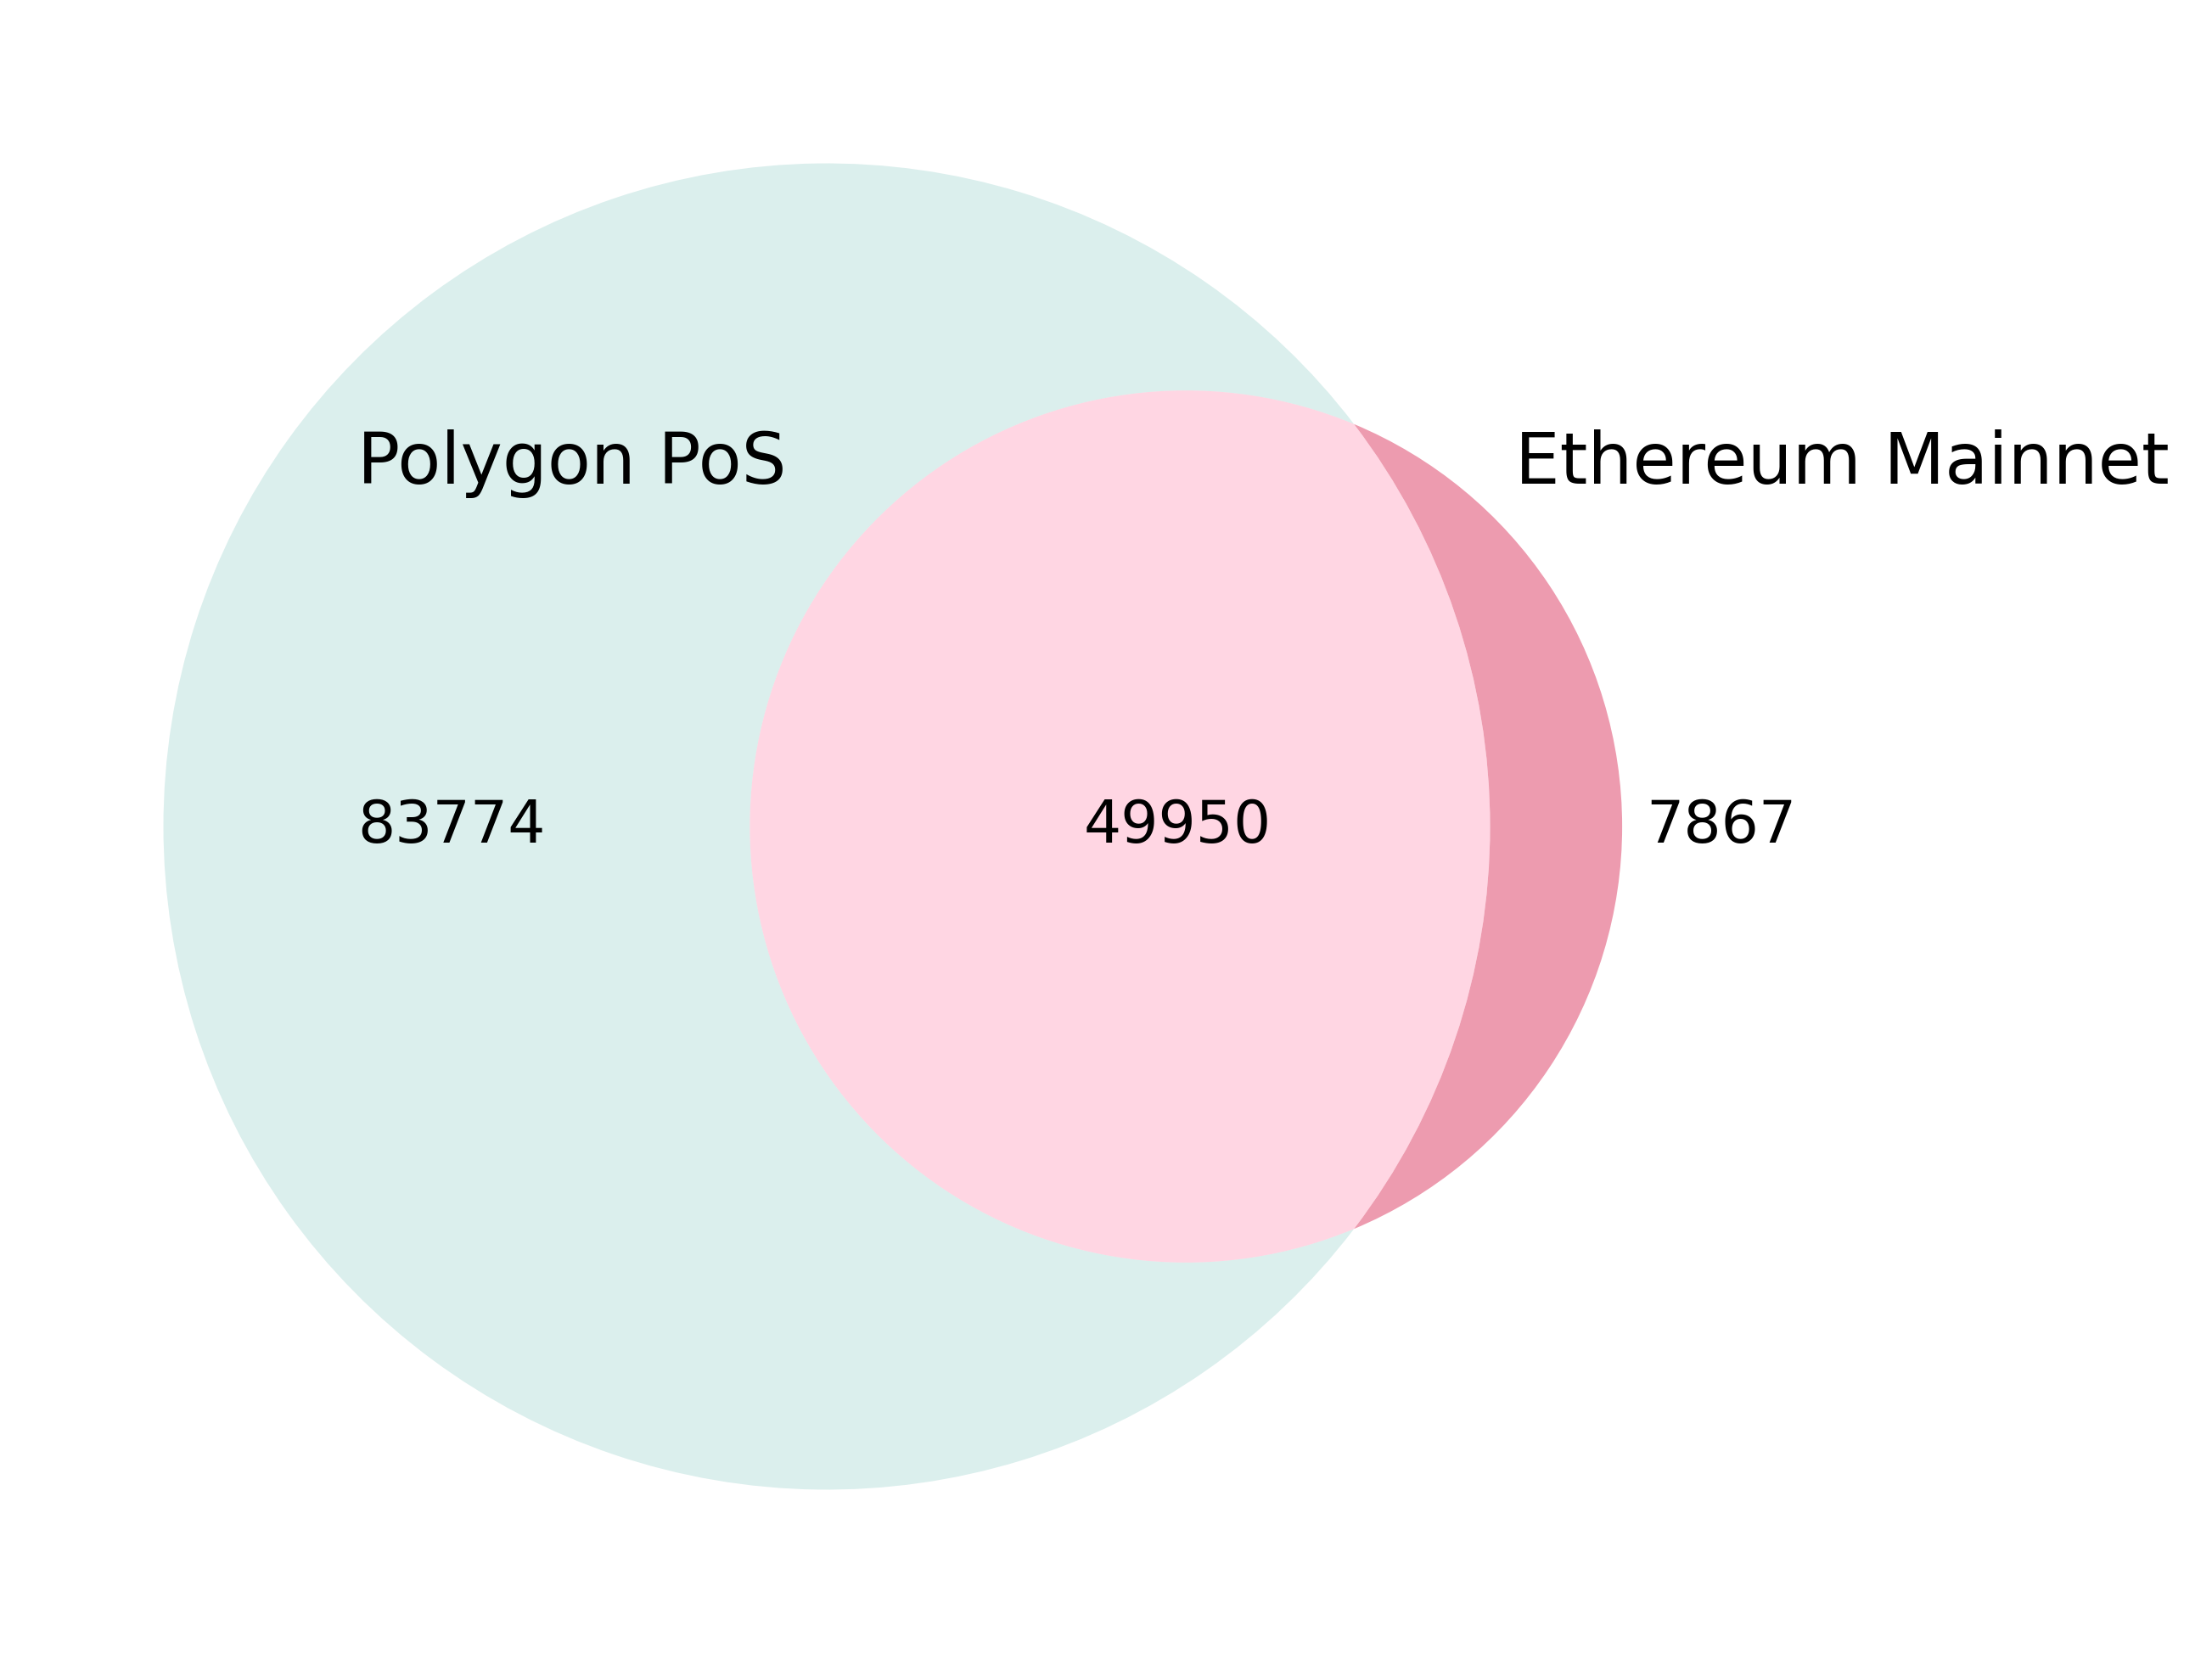
\includegraphics[width=0.6\textwidth]{../figures/venn_diagram.png}
	\caption{Address Subsets Visualized in a Venn Diagram}
	\label{fig:Venn}
\end{figure} 

\subsection{Transactions and Token Transfer Events}
The address subsets were used to collect transaction and token transfer event data from Ethereum and Polygon. Ethereum or Polygon data can be accessed directly through a node or an application programming interface (API) provider like Infura or Etherscan. The absence of account indexing in Ethereum or Polygon poses a challenge for retrieving all past transactions and token transfers of a specific address, as it requires scanning through all blocks and token transfer events emitted by designated token contracts. Fortunately, Etherscan offers an API Endpoint Module for ``Accounts`` that facilitates the retrieval of transactions and token transfer events for a given address. By using our network-specific address subsets, we were able to significantly decrease the number of required API calls. 
We gathered all transactions and token transfers up until block \texttt{17,670,000} on Ethereum (July 11, 2023) and block \texttt{44,990,000} on Polygon (July 12, 2023). In total, we collected more than 30 million %30,689,978
token transfer events and more than 16 million %16,092,531
 normal transactions. While the amount of transactions is similar between the two networks, Polygon has roughly three times more transfer events. \newline The output was stored in separate CSV files and also imported into a MongoDB\footnote{\url{https://www.mongodb.com/}} database. The database contains distinct collections for transactions and transfers. For additional information on the data fields of each collection, see Appendix. 
 

\iffalse
Transfer Events: 30,689,978
Transfer Events Ethereum: 7,832,778
Transfer Events Polygon: 22,857,200

Transactions = 16,092,531
Transactions Ethereum = 8,448,584
Transactions Polygon = 7,643,947

Figure X visualizes the number of daily transactions and token transfers for each chain.
\begin{figure}[h!]
	\centering
	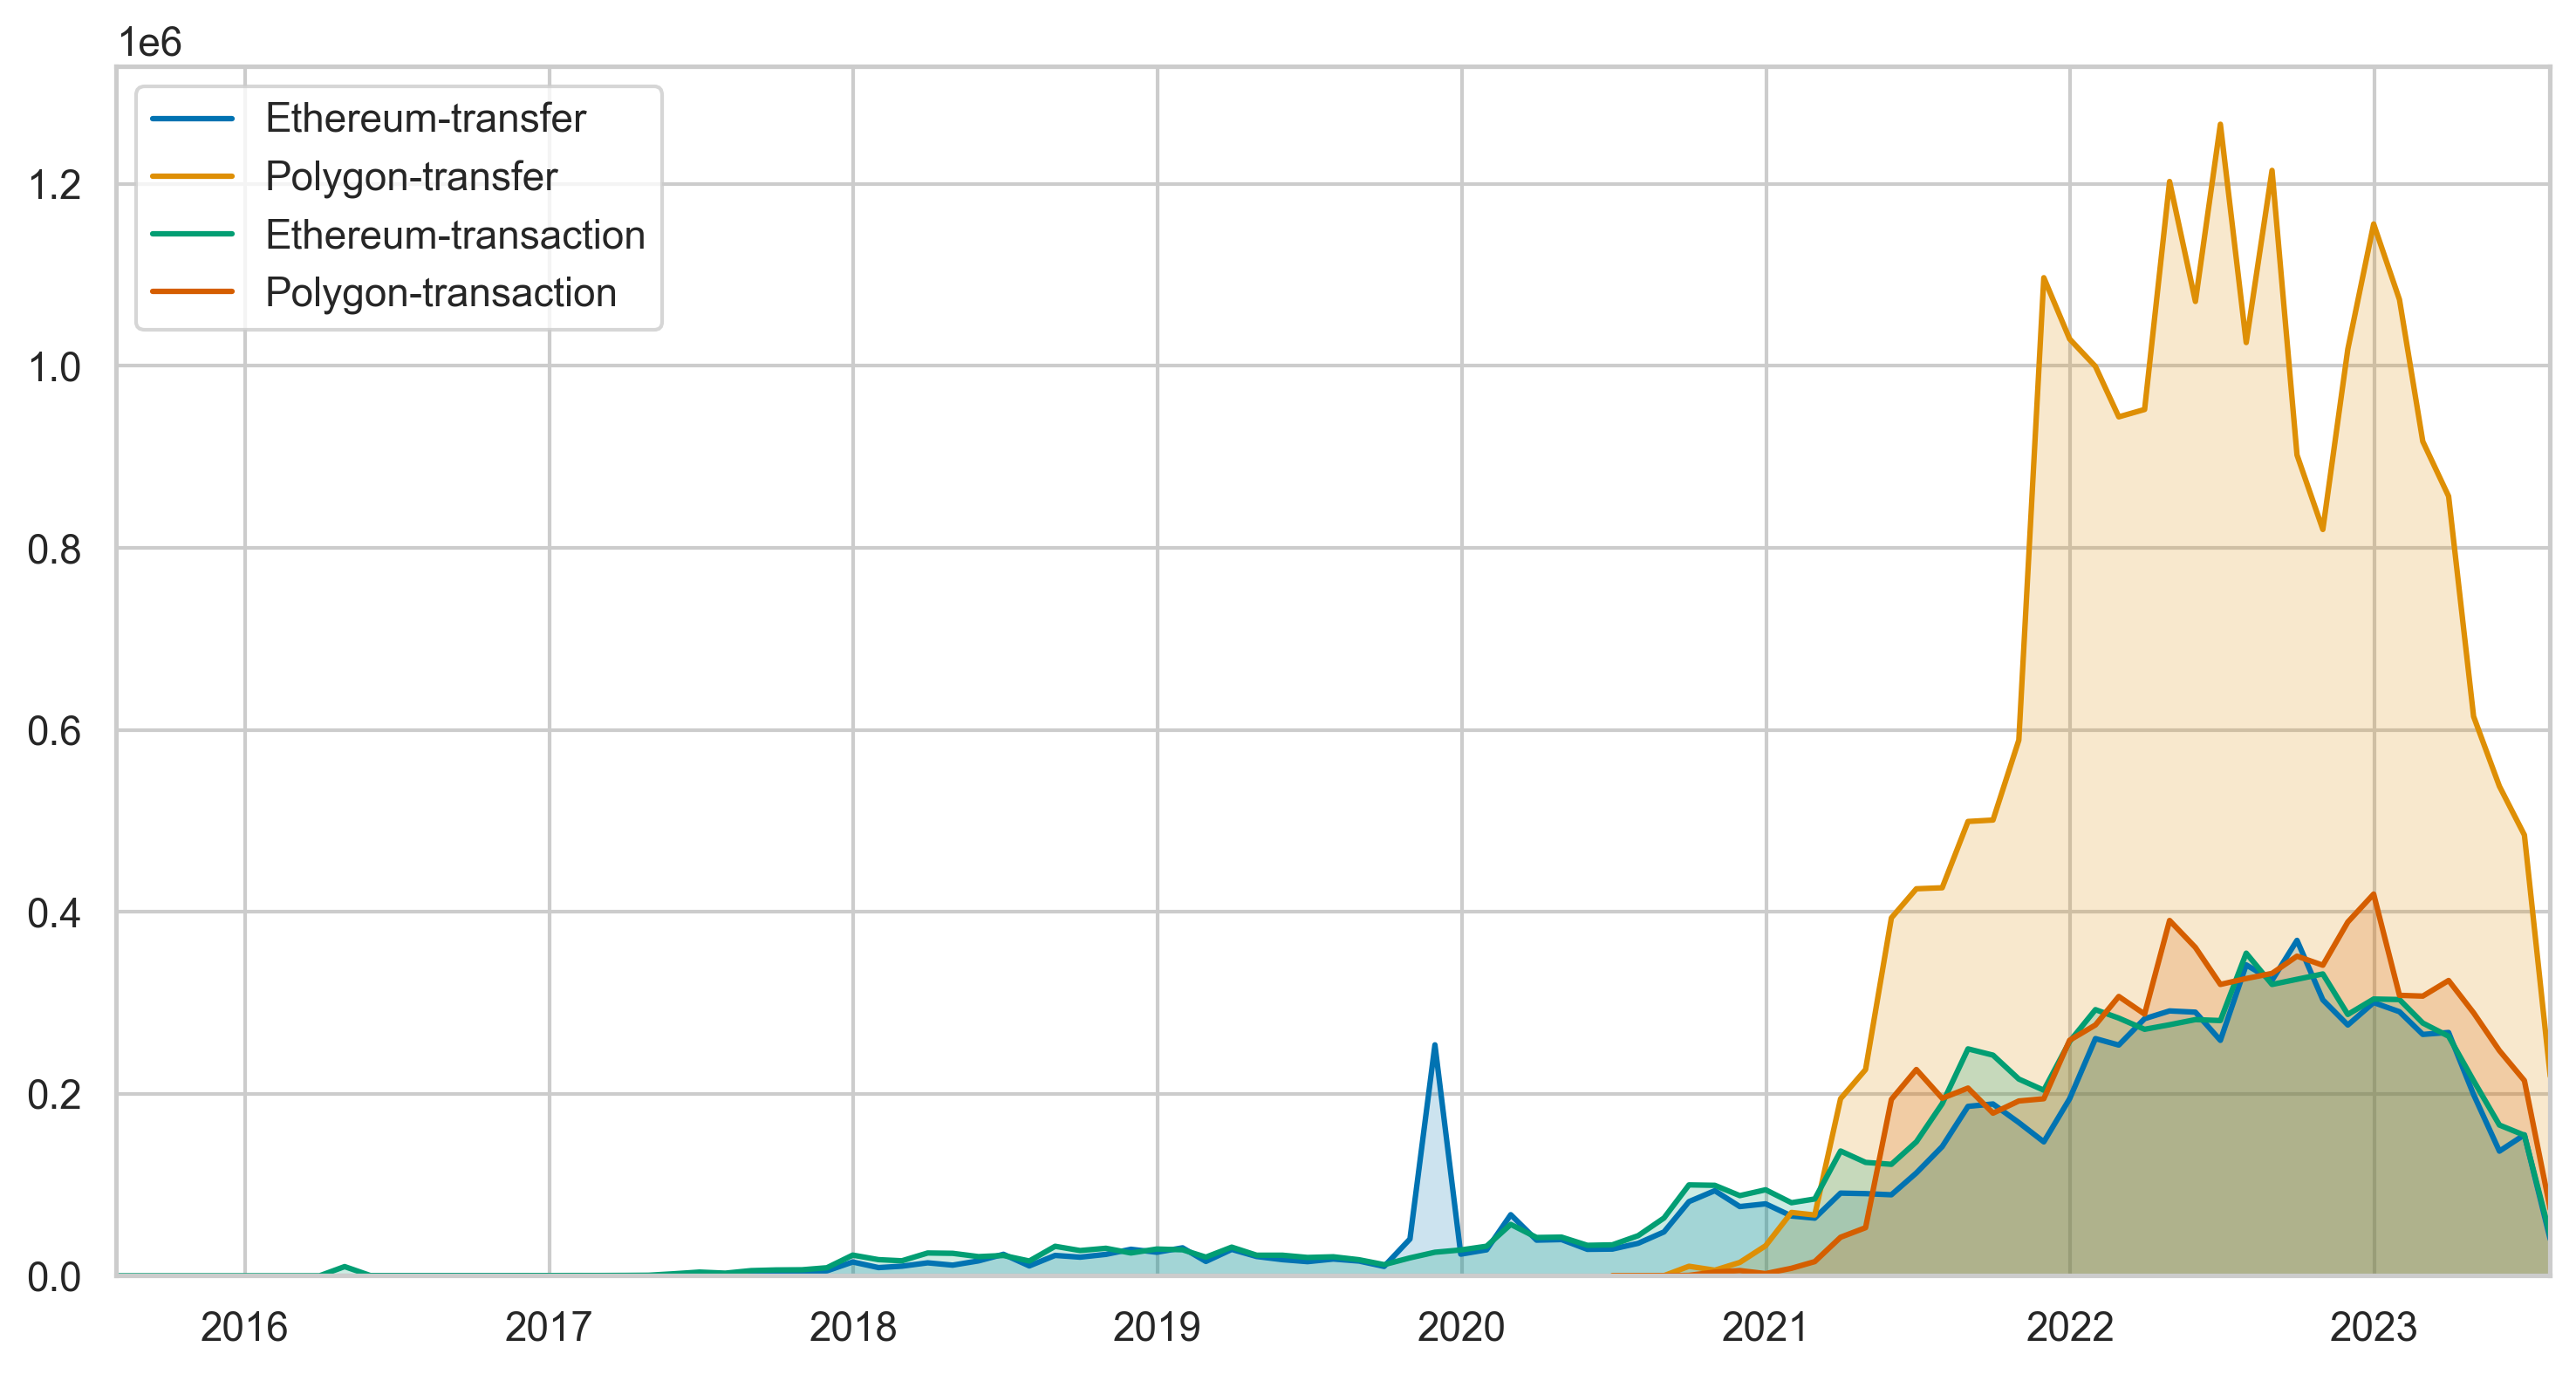
\includegraphics[width=\textwidth]{../figures/transfers_tx_by_chain.png}
	\caption{Monthly Transactions and Token Transfers by chain}
	\label{fig:Data}
\end{figure} 
Transfer Events, adding Information (isInSet) \\
Transactions \\
Filtering, Intra-set transfers\\
Data Structure, Fields \\
\fi


\subsection{Intra-set asset transfers}
\label{sec:intra-set}
In this thesis, we want to employ entity clustering heuristics to determine the number of entities represented by the remaining 137,544 addresses. Or, to phrase it differently, do users interact with Decentraland using multiple EOAs, and can we identify addresses that belong to the same user?
\newline
To achieve this, we often only %need to
consider transactions or token transfer events where both the ``\texttt{from}`` (sender) and the ``\texttt{to}`` (recipient) address are within the address set. We call this reduced dataset ``intra-set asset transfers``. Regarding normal transactions, this means that we only keep native asset transfers (Ether or Matic) as almost all addresses are EOAs. \newline
The intra-set asset transfer dataset is mainly used to generate the network graphs (see Section \ref{sec:node}). %used for the node embedding methods
When clustering addresses using graph-based approaches, this has the advantage that we do not need to differentiate between EOA and smart contract account later on. Furthermore, it allows us to observe and visualize the asset flows between users. In total, we have 974,478 intra-set token transfers and 210,548 intra-set native asset transfers (101,621 Matic, 108,927 Ether).

\iffalse
%further simplifies the clustering process. \newline
%(logging in to Decentraland with multiple addresses) When it comes to entity clustering, we essentially want to answer the question of how many real-world entities our remaining  137,544 addresses represent. 
-Also for other clustering heuristics we often make this reduction, for example: In the self-approval approach, we only consider approval transactions where another address from the set is approved.
-filter our transactions and token transfers to entries where both the 'from' and the 'to' are within this narrowed pool of addresses. We define this as intra-set asset transfers. For the transactions, this means that we only consider native asset (Ether or matic) transfers. %between two EOAs
-As already mentioned in the introduction, the goal of this paper is to cluster addresses within who (1) were active in Decentraland during the 9-month period (e.g., within the initial dataset) and (2) transacted or interacted with any token on Ethereum or Polygon. 
-Essentialy, we want to answer two main research questions when it comes to clustering:
1. How many unique entities does the address set represent (i.e. were active on Decentraland during the 9-month period)?
2. Are users interacting through multiple accounts/EOAs/addresses with Decentraland?
-we focus on on-chain data (and not user location or avatar data), allowing us to exclude addresses that have not transacted or interacted with any token on Ethereum or Polygon. 
-As mentioned in the introduction, the goal of this paper is to cluster addresses belongig to the same entity that were recorded/active in Decentraland during the 9-month period. Therefore, we disregard addresses outside of this set. Also, since we only look at on-chain data, we cannot cluster addresses without activity on Polygon or Ethereum. Doing these two reductions, there are  141, 591 'clusterable' addresses remaining.
-Since all of our addresses are EOAs (some multisig smart contract wallets). -> Check this?
\fi

\subsection{ENS ground-truth pairs}
\label{sec:ens}
Similarly to \cite{Beres2020}, we use Ethereum Name Service (ENS) identifiers as ground truth information to evaluate some of the clustering methods.\newline
\textit{ENS} is a naming system that relies on the Ethereum smart contracts. Its main purpose is to map human-readable names, such as \texttt{`alice.eth`}, to machine-readable identifiers, mostly Ethereum addresses. The architecture of ENS comprises two main components: the registry and resolvers. \newline
The \textit{ENS registry} consists of a single smart contract\footnote{The registry contract is ERC-721 compliant, which means that .eth registrations can be transferred in the same way as other NFTs.} that maintains a list of all domains and subdomains, recording the ``owner`` and ``resolver`` for each. The registry allows the owner of a domain to make changes to that data. \citep{ENSdocs} %Domain owners may set the resolver for the domain.
\newline
\textit{Resolvers} are responsible for %(the actual process of)
 translating names into addresses. Any contract that adheres to the relevant standards may act as a resolver. The process of resolving a name involves two steps: \textit{First}, the registry must be queried to find out which resolver is responsible for the name, and \textit{second}, that resolver must be asked for the response to the query. \newline
In addition to regular resolution from name to address, ENS also supports ``reverse resolution``, allowing for a mapping from address back to a name (or other metadata). Reverse resolution is accomplished via %special
 domain \texttt{`addr.reverse`}% and the resolver function \texttt{name()}.
. This domain is owned by a special purpose registrar contract that allocates subdomains to the owner of the matching address - for instance, the address \texttt{`0x1234\dots`} may claim the name \texttt{`1234\dots.addr.reverse`}, and configure a resolver and records on it. The resolver in turn supports the \texttt{name()} function, which returns the name associated with that address.\newline
 Reverse resolution %(without a library)
 follows the same pattern as forward resolution: Get the resolver for \texttt{`1234....addr.reverse'} (where \texttt{`1234...`} is the address you want to reverse-resolve), and call the \texttt{name()} function on that resolver. However, ENS does not enforce the accuracy of reverse records. This means \texttt{`1234....addr.reverse`} may falsely claim that the name associated to their address is \texttt{`alice.eth`}. 
 
Figure \ref{fig:ENS} illustrates the mechanism that allowed us to generate ground truth pairs in a simplified way: Initially, the domain name \texttt{`foo.eth`} resolves to address \texttt{`0xABC...`}. The owner has also set a reverse resolution for this address, indicated by the the edge from the address to the domain name. Next, the owner decides to change the resolved address to \texttt{`0xDEF...`}, again setting a reverse record.  As a domain can only point to one address at the time, the previous mapping from \texttt{`foo.eth`} to the old address is deleted. However, \texttt{`ABC....addr.reverse`} still points to \texttt{`foo.eth`} and when we query the name corresponding to \texttt{`0xABC...`} and \texttt{`0xDEF...`}, both will return \texttt{`foo.eth`}.
If this special case occurs, we assume that both addresses belong to the same entity.
%We did not observe cases where someone set a reverse record to a completely unrelated address (e.g. alice.eth)

\begin{figure*}[h!]
	\begin{center}
		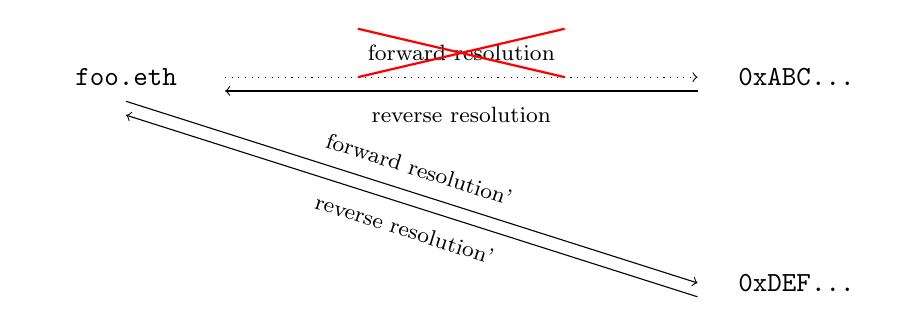
\begin{tikzpicture}[
    every node/.style={minimum width=2.5cm, minimum height=0.6cm, align=center},
    every path/.style={->},
    node distance=2cm and 6cm]

		\node (A) {\texttt{foo.eth}};
		\node[right=of A] (B) {\texttt{0xABC...}};
		\node[below=of B] (C) {\texttt{0xDEF...}};
		
		\draw[dotted] (A) -- (B) node[midway, above, name=pathAB] {\footnotesize{forward resolution}};
		\draw ([yshift=-5pt]B.west) -- ([yshift=-5pt]A.east) node[midway, below] {\footnotesize{reverse resolution}};
		\draw (A.south) -- (C.west) node[midway, sloped, above] {\footnotesize{forward resolution'}};
		\draw ([yshift=-5pt]C.west) -- ([yshift=-5pt]A.south) node[midway, sloped, below] {\footnotesize{reverse resolution'}}; 	
		
		% Adding a cross over "forward resolution"
        \draw[red, thick, -] (pathAB.south west) -- (pathAB.north east);
        \draw[red, thick, -] (pathAB.south east) -- (pathAB.north west);
							
		\end{tikzpicture}
		\caption{Changing the record to another address does not change the old reverse resolution (Simplified Schematic Representation)}
		\label{fig:ENS}
	\end{center}
\end{figure*}

We applied the following methodology to find ground truth pairs: First, we gathered all addresses that interacted with ENS (NFTs) to reduce the amount of name look-ups. Second, we iterated over each remaining address and checked if it reverse-resolved to an ENS domain\footnote{This was done via the ENS module within web3.py \url{https://web3py.readthedocs.io/en/stable/ens_overview.html}, which provides an interface to look up domains and addresses.}. If so, we logged the ENS domain and address in a CSV file. Third, using our new list, we identified if two addresses referenced the same ENS domain. If matched, we recorded both addresses alongside the ENS domain. \newline
From this, we identified 11,440 reverse records and 40 address pairs, %(addresses pointing to the same .eth name)
which we utilized as our ground truth to evaluate various clustering heuristics. Although this sample is relatively small, it allows us to assess and draw conclusions about the effectiveness of the methods.%profiling techniques/methods

\iffalse
-Check for each address in the list if the address points to an human-readable name. (reverse mapping must be set/configured) From the web3.py documentation \url{https://web3py.readthedocs.io/en/stable/ens_overview.html } %The ens module is included with web3.py. It provides an interface to look up domains and addresses, add resolver records, or get and set metadata.
-If two addresses point to the same ENS name we consider them belonging to the same entity. 
-Normally, one .eth domain cannot point/map to multiple Ethereum addresses. Forward resolution. This is likely due to the owner change and the record not updated.

%However, if someone sets the forward resolution to a new address (owner) including a reverse resolution for his ENS name, the (reverse) resolution from 0x05d.addr.reverse still resolves to the the ENS domain name.
%Only the forward resolution from the name to the address is changed. The reverse record resolution from the old address to the name is still there. For an visual explanation please see Figure \ref{fig:ENS}.
%In addition to regular resolution from name to address, ENS also supports ``reverse resolution``, making it possible to map from address back to a name (or other metadata).
%Anyone who owns a domain at any level may configure subdomains - for themselves or others - as desired. For instance, if Alice owns 'alice.eth', she can create 'pay.alice.eth' and configure it as she wishes.
%Currently, all the subdomains or non .eth domains are not NFTs, unless the domain registrar itself supports NFT such as (dcl.eth, and .kred).
%If the owner sets a reverse resolution set with his new address, we have two addresses pointing to the same ens name. 

%While 'regular' resolution involves mapping from a name to an address, reverse resolution maps from an address back to a name - or other metadata. ENS supports reverse resolution to allow applications to display ENS names in place of hexadecimal addresses. Before this can be done, the owner of the address has to configure reverse resolution for their address.
%In spirit, it is similar to the well-known Domain Name Service (DNS). However, in ENS the registry is implemented in Ethereum smart contracts.
%Therefore, ENS provides a more user-friendly way of transferring assets on Ethereum, where users can use ENS names as recipient addresses instead of the error-prone hexadecimal Ethereum addresses.
%Resolving a name is a two-step process: First, ask the registry what resolver is responsible for the name, and second, ask that resolver for the answer to your query.\newline

\fi

%%%%%%%%%%%%%%%%%%%%%%%%%%%%%
%%% Clustering Heuristics %%%
%%%%%%%%%%%%%%%%%%%%%%%%%%%%%

\section{Clustering Heuristics}
In this section, we present an overview of clustering heuristics in the context of account-based blockchains and on-chain data. We will give a detailed explanation of the mechanics and rationale behind the heuristic and assess its applicability to our case. 
In Section 5, we will implement and evaluate the heuristics we determine to be suitable for our objectives.

% Goal: explain each heuristic, categorize, and discuss applicability to our address set
%In Section 5 we will then apply  and, if possible, evaluate the heuristics deemed suited for us.
%intuition

\subsection{Self-authorization} 
	All three token standards require functions to allow another address to transfer tokens on behalf of the actual owner. For the ERC-20 standard, this is achieved through the \texttt{`approve`} function, accepting the spender's address and the token amount as parameters\footnote{\texttt{approve(address spender, uint256 amount)}}. The ERC-721 has two functions dedicated to approvals: One for authorizing the transfer of a specific NFT\footnote{\texttt{approve(address to, uint256 tokenId)}} and one to permit transferring all of the owner's NFTs within the collection\footnote{\texttt{setApprovalForAll(address operator, bool approved)}}. The latter function also appears in the ERC-1155 standard. The approval functionality of these tokens is primarily used in connection with smart contracts (DEX or NFT Marketplace), but can also be applied for regular EOAs. \newline
The ``self authorization`` heuristic, proposed by \cite{FV:17}, suggests that users might authorize another address they own, possibly for risk distribution across several addresses or for testing purposes. \newline
Given our dataset includes all address transactions, we can easily employ this heuristic. %Since all the addresses' transactions are available in our dataset, we are able to apply this heuristic.


\iffalse
	For the ERC-20 standard: \texttt{approve(address spender, uint256 amount)}
	For the ERC-721 standard: \texttt{approve(address to, uint256 tokenId)} and \texttt{setApprovalForAll(address operator, bool approved)}\\
	For the ERC-1155 standard: \texttt{setApprovalForAll(address operator, bool approved)}
	
	- approve(address,uint256)
	- setApprovalForAll(address,bool) for both ERC-721 and ERC-1155
	
The first step is to get all approval transactions. We achieve this using the 'input'/calldata field. The first X bytes are always the function selector. We filter for the known function selectors for all standards. Next, we get the approved address/spender, also from the calldata, it is always at the same spot. We filter for spenders within the address set and for spenders who are different from the 'from' address. How many transactions are remaining? Finally, we extract all unique pairs of owners and spenders, disregarding the type of token or the amount.
\fi


\subsection{Deposit address reuse}
The concept of deposit address reuse was first introduced and systematically utilized by \cite{FV:17} and subsequently adoped by \cite{wu2022tutela}. This heuristic relies on the prevalent practice of crypto exchanges generating unique deposit addresses for each user. These addresses then forward the funds to an exchange's main address. It is highly likely that multiple addresses sending funds to the same deposit address are controlled by the same entity. They key challenge of this approach lies in identifying these deposit addresses, which could either be EOAs or smart contracts. \newline
Deposit addresses share the characteristic that they forward the received funds to a major exchange account. Two parameters are essential for deposit address detection: the discrepancy between the amount received and forwarded (since the exchange must pay gas fees), and the time lag between receiving and forwarding funds.
However, our dataset only includes the direct transactions or token transfers associated with the addresses. The transactions between deposit and main exchange address are absent. Consequently, this clustering heuristic is not applicable to our data.


\iffalse
\cite{FV:17} was the first to formulate and systematically exploit this heuristic, which was also applied later on by \cite{wu2022tutela}. This heuristic exploits the common practice of crypto exchanges creating so-called deposit addresses for each user, which forward funds to a main address. Multiple addresses that send funds to the same deposit address are highly likely controlled by the same entity. The main challenge of this approach is detecting deposit addresses, which can be either EOAs but also smart contracts.
- Exchanges typically create so-called deposit addresses, which will forward received funds to a main address. As these deposit addresses are created per customer, multiple addresses that send funds to the same deposit address are highly likely to be controlled by the same entity. 
The key challeng lies in identifying these deposit addresses. Their characteristic property is that they forward received amounts to a major exchange account. The forwarded amount is often slightly less than what was received, as the exchange has to pay for the transaction costs. In most cases, deposit addresses are EOAs, but they can also be smart contracts. Identifying deposit addresses relies on two parameters: the maximum amount difference between what was received and forwarded and the maximum time difference between receiving and forwarding.
In this project, we only collected the addresses' direct transactions or token transfers. This would allow us to see deposit addresses, however, with this data we cannot find the second step: the deposit address forwarding the asset to the exchanges main address. Therefore, we do not apply this clustering heuristic here.
Since we only collected the addresses' direct transactions or token transfers, the second step between deposit and exchange address is not available/present in our dataset. 
\fi

\subsection{Airdrop multi participation}
Airdrops are popular token distribution mechanisms, and recipients are mostly chosen based on past protocol activity. Probably the most well known example is Uniswap's UNI airdrop, where each address that interacted with the protocol until a specified cutoff date received a fixed amount of 400 UNI tokens\footnote{\url{https://blog.uniswap.org/uni}}. Especially in the early days of airdrops, these distribution mechanisms were not Sybil-resistant, leading to people creating multiple addresses in anticipation of an airdrop. However, \cite{FV:17} argues that managing the tokens on all of these addresses is impractical, which is why they are often aggregated into one address. He finds around 500 same-source, fixed amount token distribution events with at least 1,000 recipients while also taking into account the block difference between the individual aidrop token transfers. He defines multi-participation when two airdrop recipients forward their tokens to a single address. Since we do not have a whole view of the airdrop distribution events, we are not able to find them using our data. One possible approach would be to manually select known airdrops. However, this process takes very long and is not guaranteed to cluster a lot of addresses, since most new airdrop events were made with some kind of sybil-resistance. Nevertheless, to test this approach we searched for addresses that forwarded the UNI airdrop to another address. We found X addresses that did that, but no two addresses forwarding the amount to a third address.

\iffalse
Airdrops are a popular mechanism to distribute tokens. On the Ethereum blockchain, they are performed through smart contracts. The owners of the smart contract choose recipients either based on past activity, or ask users to sign up through online forms. Some of these registration processes require users to perform certain actions on social media, such as posting articles or following users. The amount of tokens given to each user is either fixed, or based on existing account balances. If the amount is fixed, there is an incentive to cheat the system. 
We identify Airdrops where a fixed number of tokens is distributed to many recipients. Then we search for addresses that have been forwarded the same amount from the initial recipients. 
This heuristic depends on two inputs. First, a set of aidrops with equal mounts, characterized by a signature of a distributing address, a token network and an amount. Second, the minimum nuber of token aggregations into a single address. The second parameter is trivial to choose, as multi-participation in its smallest form consist of two aidrop recipient addresses forwarding their tokens to a third adddress. In this case, a single entity would be in control of at least 3 addresses.
The main challenge lies in identying airdrops. To do so, we first examine all same-source, fixed amount token distributions.
\fi

\subsection{Node embeddings}
\label{sec:node}

According to \cite{Beres2020}, \textit{node embedding} methods form a class of network representation learning\footnote{Sometimes also referred to as ``graph representation learning``} methods that map graph nodes to vectors in a low-dimensional vector space. These methods aim to represent vertices with similar neighborhood structure by vectors that are close in the vector space. \newline
\cite{Beres2020} first introduced this approach on a Ethereum transaction graph for the purpose of entity identification to pair Ethereum addresses associated with Tornado cash deposits and withdrawals. Building on this, \cite{wu2022tutela} refined and expanded one particular node embedding method to deanonymize Ethereum users at scale. \newline
The foundation for these node-embedding methods is an undirected graph where nodes are composed of distinct addresses, and an edge is placed between two nodes if there is a transaction between them. \newline
To construct the network graph, we use the intra-set asset transfers described in section \ref{sec:intra-set}. This approach differs from the methodologies adopted by \cite{Beres2020} and \cite{wu2022tutela}. On one hand, \cite{Beres2020} collected all transactions and token transfer events of their address set, but did not refine this data to only include intra-set asset transfers. On the other hand, \cite{wu2022tutela} do not operate on a specific address set, but use all Ethereum transactions to build the network graph, ignoring token transfer events. \newline %vielleicht erklären wieso wir es anders gemacht haben
Using the network graph, node embedding methods seek to learn a function that projects a node to a $d$-dimensional vector representation (also called feature vector). This is a way of simplifying the graph information by associating each node with a point in the Euclidean space. Various node embedding methods have been developed and applied to different domains. \citep{rozemberczki2020difftovec} \newline
The intuition behind node-embedding approaches is that addresses which interact with the same set of addresses within the network graph should be close in Euclidean distance. \cite{Beres2020} cites two main reasons for this. Firstly, users with multiple accounts often interact with the same addresses or services from most of them. Secondly, when users move funds between their personal addresses, they may unintentionally reveal their address clusters. \newline
\cite{karateclub} provide a variety of node embedding methods as a Python library\footnote{\url{https://github.com/benedekrozemberczki/karateclub}}. They categorize the methods into neighborhood (proximity) preserving and structural. \newline
We focus on the three methods that performed best in \cite{Beres2020} experiments: ``Diff2Vec`` \citep{rozemberczki2020difftovec}, ``Role2Vec`` \citep{ahmed2018roletovec}, and ``Deepwalk`` \citep{perozzi2014}. Diff2Vec and DeepWalk are both neighborhood preserving, while Role2Vec is a structural node embedding method. Although all of these methods utilize random walks to capture graph information, they differ in their approaches to leveraging these random walks for constructing Euclidean feature vectors. A detailed explanation of each method is beyond the scope of this thesis. For a concise overview of Diff2Vec, please refer to \cite{wu2022tutela}. The interested reader may consult the originial publications. \newline
With our intra-set asset transfer data (\ref{sec:intra-set}) and ENS address pairs (\ref{sec:ens}), we were able to apply and evaluate the node embedding methods described above. Using the library described by \cite{karateclub} requires certain preprocessing steps for the network graph. Transactions must be treated as undirected edges and loops (self-transactions) and multi-edges should be removed. Moreover, nodes outside the largest connected component are excluded. The resulting network graph includes 51,566 nodes and 249,302 edges. \newline
It is worth noting that unlike \cite{wu2022tutela}, we decided not to include edge weights. For instance, if Alice sent Bob Ether three times and Bob sent Alice Ether two times, the edge weight would correspond to five. This choice facilitated the application of \cite{rozemberczki2020difftovec}'s library and eliminated the need to create a custom method. \newline
Based on our network graph, we generate 128-dimensional feature vectors for each address and method. \newline
Given an node embedding, we can search for the closest $k$ vectors to any given vector. As in \cite{wu2022tutela}, we accomplish this using FAISS (Facebook AI Similarity Search), developed by \cite{johnson2019faiss}, which always returns a list of $k$ nodes, ranked by their Euclidean distance to the given node\footnote{We set $k = 51566$, the total number of nodes in the network graph}. \newline
To evaluate the three node embedding algorithms, we use our ENS address pairs as ground truth. We run each node embedding method ten times and report the average rank of the target address. For comparison, we  compute the mean, median and standard deviation of the average rank for each method.

\iffalse
\textbf{Diff2Vec} % Neighborhood preserving 
The intuition of Diff2Vec is to summarize a node by its neighborhood through a diffusion-like random process. Specifically, there are four steps to Diff2Vec: 1) Generating a diffusion graph, 2) sampling a node sequence, 3) extracting features, 4) learning a neural network embedding
\textbf{DeepWalk}
\textbf{Role2Vec} % Structural node embedding, Structural Node Level Embedding
Random walks will likely visit nearby vertices first, which makes them
suitable for finding communities, rather than roles (structural
similarity). To overcome the above problems, we propose the Role2Vec
framework which serves as a basis for generalizing many existing methods that use traditional random walks. Strucural feature matrix.

Research in node embedding has been accelerated by Word2Vec, which is an embedding method for natural language processing. This approach has been extended to learn graph/network embeddings.

Token networks -> Victor, Casale Brunet
\fi


\subsection{Time-of-day transaction activity and gas price selection}

Apart from the node embedding methods applied to Ethereum transaction graphs, \cite{Beres2020} suggest employing clustering heuristics based on time-of-day transaction activity and gas price distribution. \newline
\textit{Time-of-day transaction activity} considers all transaction timestamps initiated by a particular address. These UNIX timestamps are transformed into hour-of-the-day-based values. The authors argue that account owners may expose daily activity patterns and represent addresses by a vector including the mean, median and standard deviation, as well as an activity histogram divided into 4-6 hour bins \citep{Beres2020}.  Figure \ref{fig:ToD} illustrates the time-of-day activity histogram and kde for a selected ENS address pair, divided into two hour intervals.\newline
Additionaly, the \textit{gas price distribution} heuristic leverages the possibility of users revealing patterns when choosing their gas price. Prior to EIP-1559\footnote{\url{https://eips.ethereum.org/EIPS/eip-1559}}, users could set the gas price manually. In practice, most wallet user interfaces offered three levels of gas prices: slow, average, and fast. Selecting the the fast option would ensure almost immediate inclusion in the blockchain. To account for the changes in Ethereum traffic volume, the gas price is normalized by the daily network average. The combination of gas price levels that a user select forms their personal gas price profile. An account is represented by a vector including the mean, median, and standard deviation and a normalized gas price histogram divided into 50 bins, which they determined to be optimal for clustering performance. \citep{Beres2020} \newline
We will not employ both methods due to their significantly poorer performance compared to node embeddings. Nevertheless, we test a two-step approach: In the first step, we implemented Diff2Vec to find the 10 nearest neighbors. In the second step, we ordered the remaining addresses by their Euclidean distance derived from the time-of-day and/or gas price feature vectors. We analyzed the impact of this two-step approach on the average rank of a target address.

\begin{figure}[h!]
	\centering
	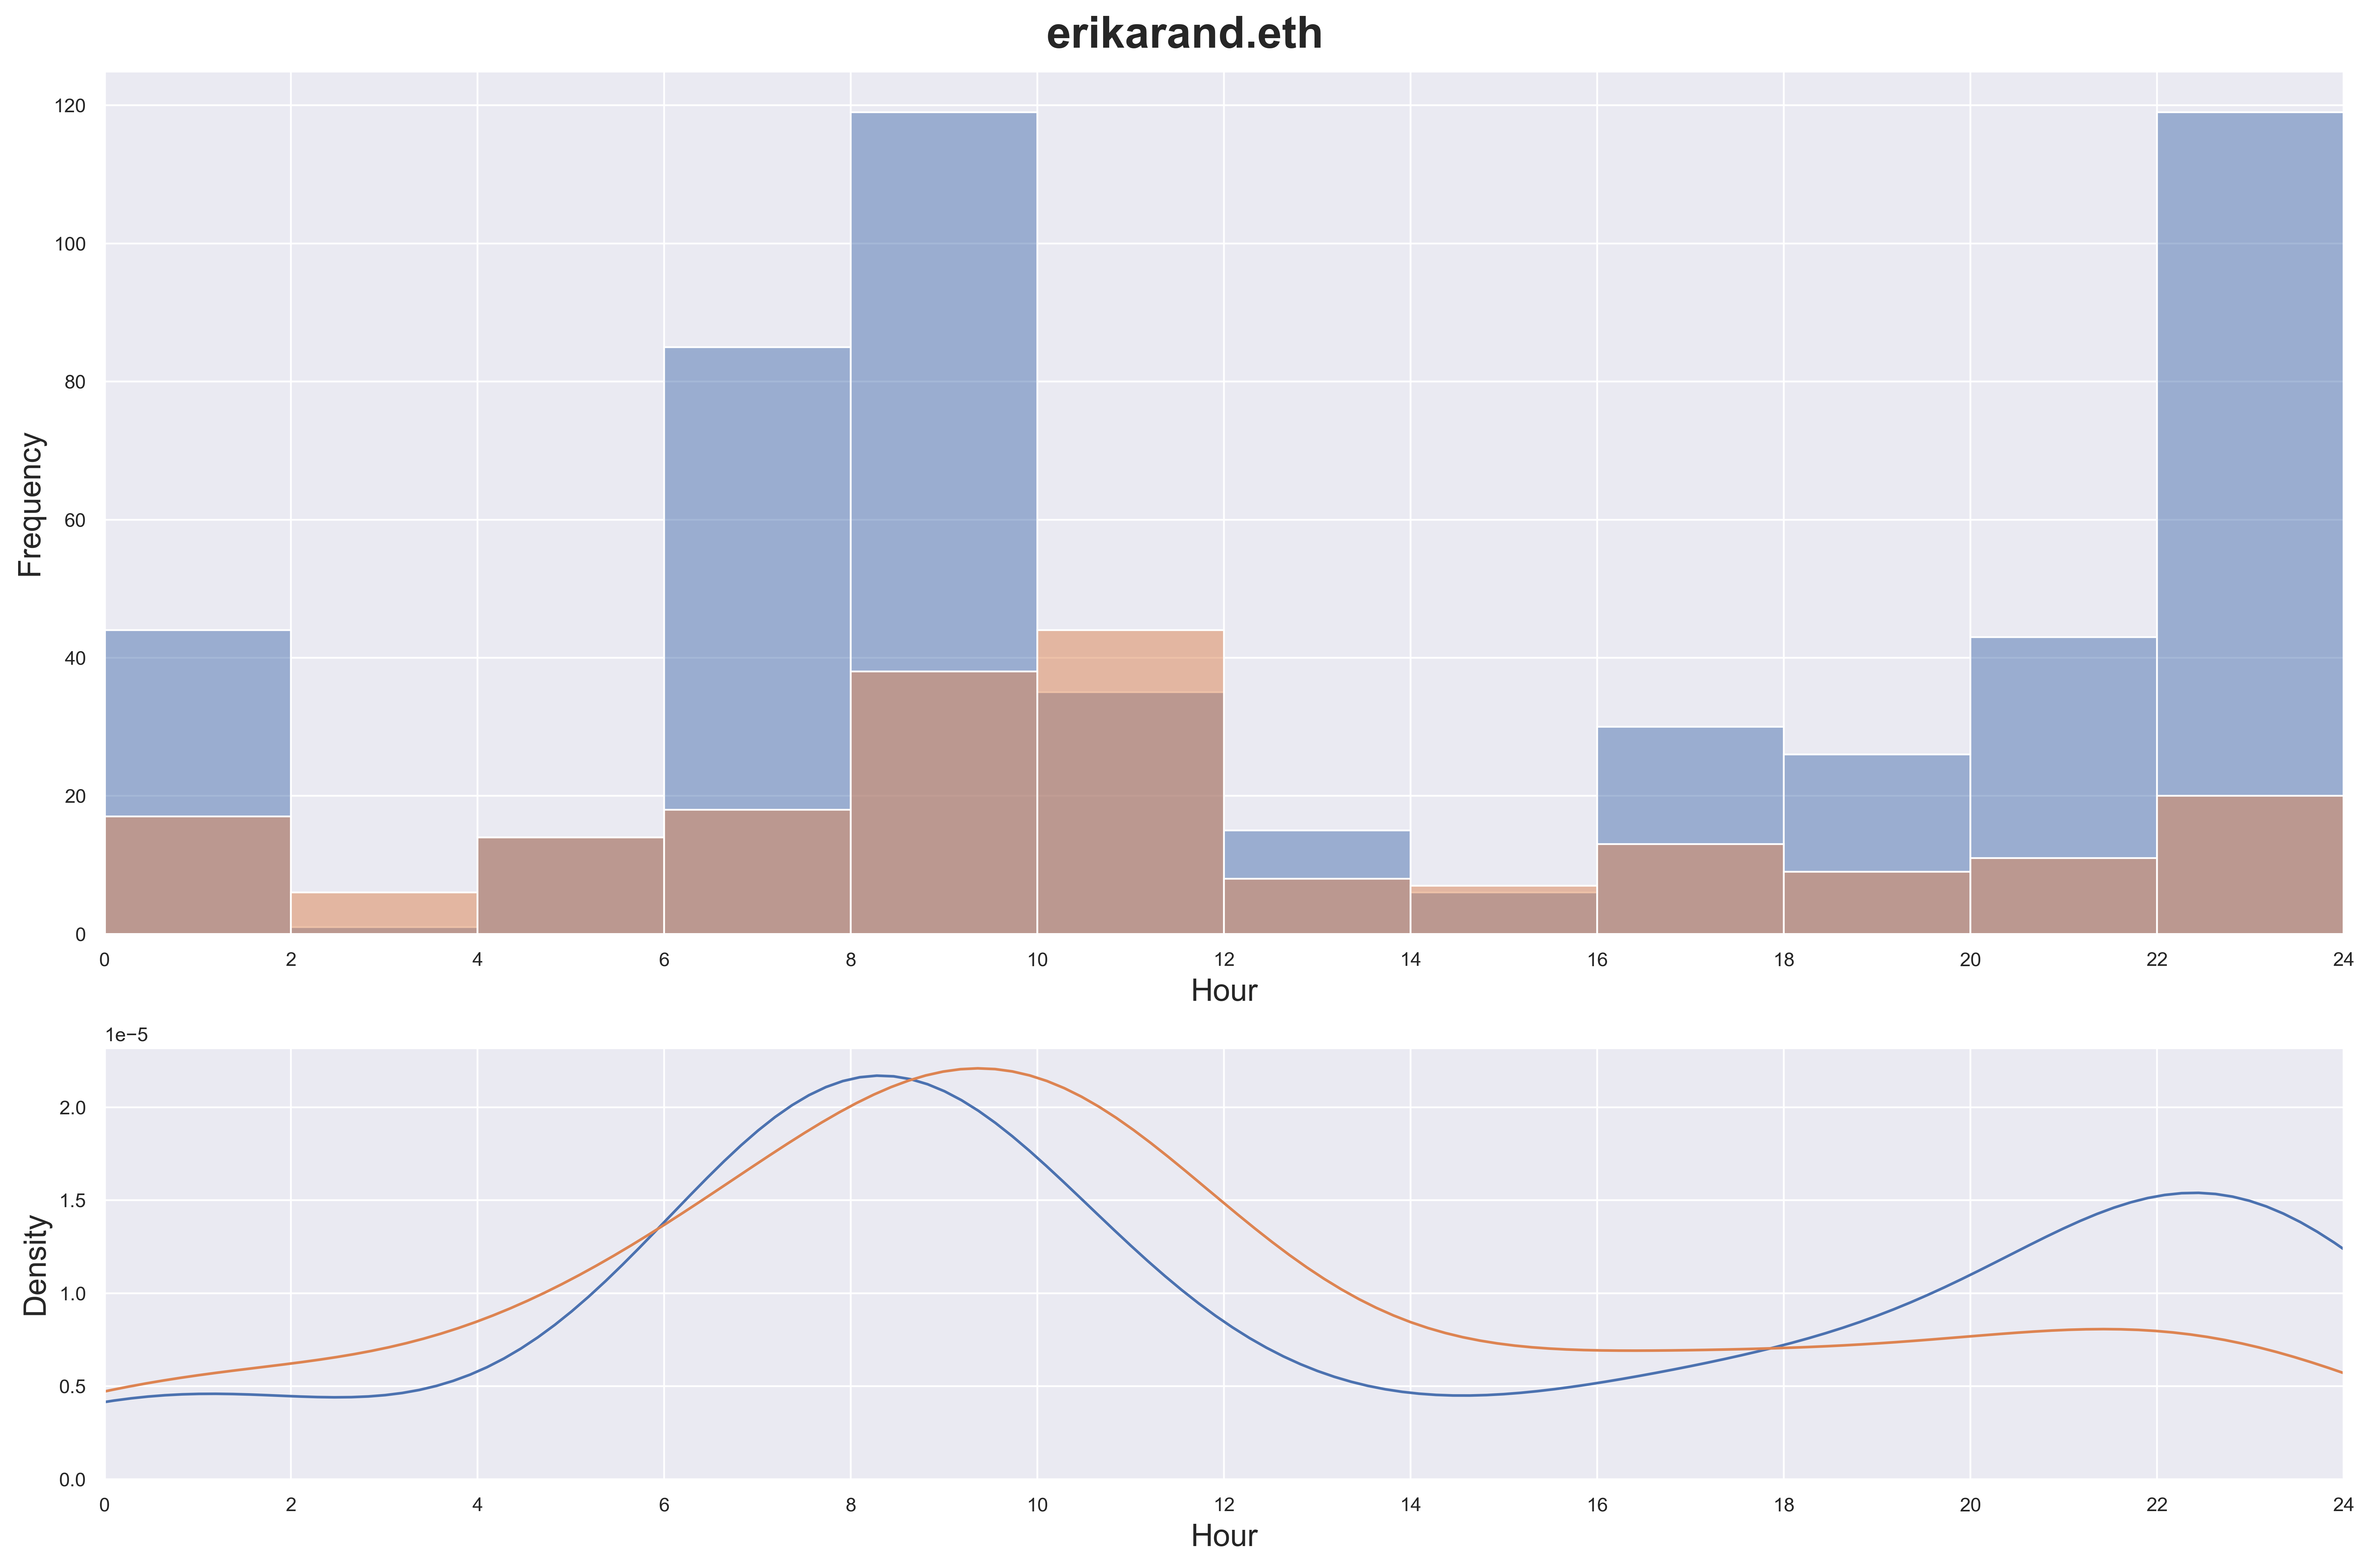
\includegraphics[width=0.8\textwidth]{../figures/time-of-day-activity.png}
	\caption{Time-of-day activity histogram and kde}
	\label{fig:ToD}
\end{figure} 

\subsection{Tornado cash heuristics}

\cite{wu2022tutela} proposed five heuristics targeted at Tornado cash, highlighting that careless user behavior can still reveal identity, despite using a mixer. The heuristics they identified are as follows: \newline
``Address match`` refers to instances where individuals use the same address for both depositing and withdrawing from the Tornado pool. ``Unique gas price`` involves users selecting a distinct (specific) gas price for both their deposit and withdrawal transactions (prior to EIP-1559). ``Linked ETH addresses`` examines whether a deposit address has interacted with a withdrawal address outside of Tornado Cash. ``Multiple denomination`` assesses an address' transaction history; two addresses with matching deposit and withdrawal portfolios are considered a pair. ``Torn minting`` identifies a specific user behavior when withdrawing so-called Anonymity points, an incentive scheme reward for increasing the anonymity set when depositing assets into Tornado cash.

We identified 84 transactions tied to Tornado cash pools, including 72 deposits, 10 withdrawals, and two transactions where the same address sent 0.1 Ether to the corresponding pool without invoking the deposit function.  Despite applying all clustering heuristics except "Torn minting," we found no clusters.

\subsection{LAND transfers}
In addition to the existing clustering heuristics, we propose our own heuristic based on transfers of high-value NFTs such as LAND. We argue that, given the high value of Decentraland land parcels, there is a high probability that addresses are controlled by the same entity when LAND is transferred without any compensation. A user might perform such transfers to rearrange their LAND holdings, e.g., by upgrading to a more secure wallet implementation. \newline
The primary challenge of this approach is to identify LAND transfers without any compensation. To accomplish this, we identify token or native asset transfers that took place within the same transaction as a LAND transfer. Upon manually examining various implementations of LAND trades on the most popular NFT marketplace contracts, we identified a pattern where the user address appears both in the from and to fields if a trade occurred. An example is shown on Figure \ref{fig:LAND_example}. 
In the case of pure LAND transfers, the sending and receiving addresses are the same for all transfers within a transaction. However, this approach does not consider other LAND trading schemes, including off-chain compensation or non-atomic (within multiple transactions) trade settlement.

\begin{figure}[h!]
	\centering
	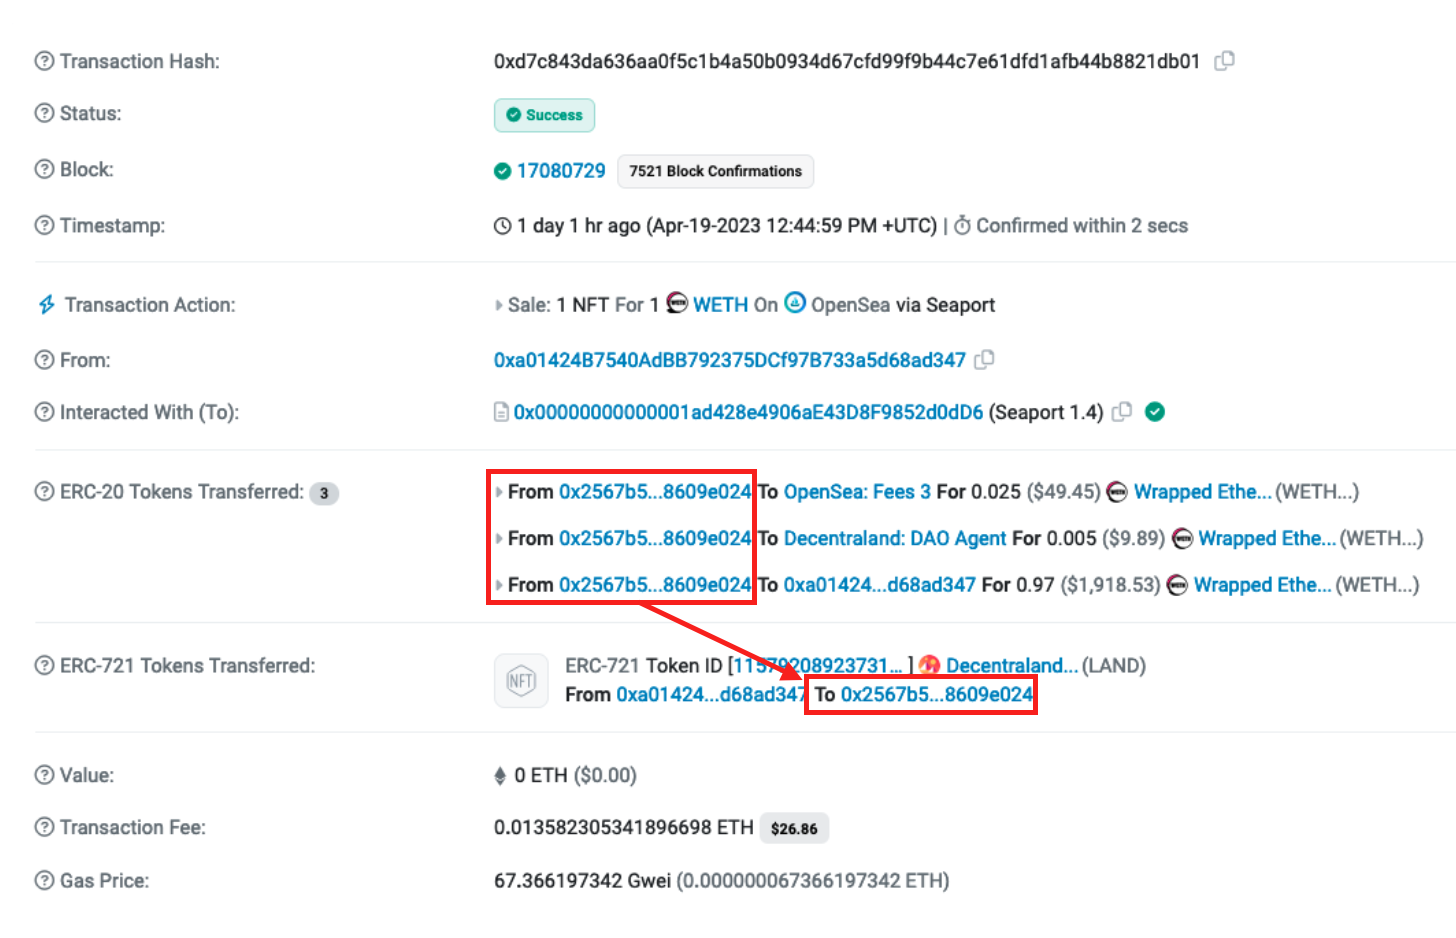
\includegraphics[width=\textwidth]{../figures/land-opensea.png}
	\caption{LAND trade on Opensea, Source: \url{https://etherscan.io/tx/0x2c2a70114e9080596bf5da6ad9c9b9f6d7e4c85a9d3b06e992f7248f9457a2ec}}
	\label{fig:LAND_example}
\end{figure} 


%%%%%%%%%%%%%%%%%%%%%
%%% Data Analysis %%%
%%%%%%%%%%%%%%%%%%%%%

\section{Data Analysis}
This section analyzes clustering heuristics applicable to our address set using the collected data. These include self-authorization, node embedding, and our proposed approach involving LAND transfers.

\subsection{Self-authorization}

For this clustering heuristic, we analyze the transaction data of the addresses, focusing on the transaction's ``calldata``. The first four bytes of the calldata represent the selector of the function signature, which specifies the smart contract function to be invoked. \newline
\textit{First}, we query all transactions that begin with a function signature related to the approval functions corresponding to ERC-20, ERC-721 and ERC-1155 token standards. This step helps us identify all approval transactions. \newline
\textit{Second}, we extract the approved address (spender address), which is always located at the same position within the calldata due to token standardization. We then record the spender address in a new field within our dataframe. \newline
\textit{Third}, we implement two filters on the approval transactions. The first filter checks if the spender address is part of our address set, and the second ensures that the spender address is different from the address initiating the transaction, thus eliminating self-approvals, which may occur due to a user interface bug or testing transactions. \newline
\textit{Fourth}, we group the remaining approvals by the initiating address and proceed to form the clusters.

We identified 16 clusters across 126 self-authorizing transactions, comprising 115 distinct addresses. After manual inspection, we excluded a cluster containing 80 addresses that had all approvals issued by the same address for the same token contract. The token contract represents a collection of wearable NFTs on Polygon called ``Renaissance King by René Mäkelä`` and may use an uncommon or potentially even faulty token minting scheme. \newline Ultimately, we discovered 35 addresses associated with 15 distinct entities.


\subsection{Node embeddings}
As described in previous sections, we tested different datasets to create the network graph using our ENS address pairs as ground truth. Der Approach ist zwar stark an Beres angelehnt, jedoch wendet er es an um pairs of deposit und withdrawal addressen zu clustern.

We found the intra-set asset transfers to perform best in terms of the average rank of a target address. 
Create network graph
Run ten separate experiments and calculate the average rank for each target address. The results of this are shown in Table X. Explain table, NaN values, within 5 nearest neighbors etc.



%1. Show that we tested different datasets to build network graph, best performing was intra-set asset transfers\\
%2. Evaluated the performance by average rank for the three methods, show results, describe how this method may be flawed/ why maybe not ideal\\

\begin{table}[h!]
\scriptsize
  \centering
  \begin{tabular}{llll}
    \hline
	\textbf{ENS domain name} & \textbf{Diff2Vec} & \textbf{Role2Vec} & \textbf{DeepWalk} \\
	\hline
	anisofim.eth & 2.5 & 6.2 & 2.7 \\
	arisalzberg.eth & 577.3 & 33.3 & 58.8 \\
	atearnz.eth & 2.8 & 2.5 & 3.3 \\
	awedjob.eth & 106.8 & 71.1 & 20.1 \\
	captvicky.eth & NaN & NaN & NaN \\
	disruptor.eth & 11.1 & 3.0 & 1.4 \\
	dragonkiller.eth & 30.7 & 1.0 & 1.0 \\
	eibriel.eth & 44.3 & 91.2 & 545.4 \\
	epdrabbit.eth & 16.3 & 10.4 & 4.1 \\
	erikarand.eth & 1.0 & 1.0 & 1.0 \\
	hyperspek.eth & 129.1 & 10.0 & 605.4 \\
	jamesmillerblog.eth & NaN & NaN & NaN \\
	jasonhsu.eth & 1.0 & 1.0 & 1.8 \\
	joeyz.eth & 1.9 & 1.0 & 1.0 \\
	keastie.eth & 10.4 & 1.0 & 18.2 \\
	linkg.eth & 4.0 & 1.0 & 10.3 \\
	lulox.eth & 4.2 & 1.5 & 27.2 \\
	maruudn.eth & 5.7 & 5.6 & 108.5 \\
	maryana.eth & 52.3 & 373.8 & 9.0 \\
	meanboss.eth & 9.0 & 9.0 & 51.8 \\
	metatiger.dcl.eth & 474.2 & 86.7 & 2.4 \\
	mgdivingnz.eth & 1.7 & 5.0 & 1.0 \\
	mrcryp.eth & 2.7 & 1.0 & 2.3 \\
	nicebhaiya.eth & 1.3 & 3.4 & 2.4 \\
	niceguy.eth & 1.0 & 1.0 & 2.2 \\
	ornellaweb3.eth & 3.7 & 2.0 & 284.0 \\
	pinkboots.eth & 16.9 & 14.4 & 2.2 \\
	remx.eth & 3.6 & 2.6 & 1.7 \\
	rileybeans.eth & 1.5 & 2.0 & 1.6 \\
	robertjames.eth & 2.7 & 1.0 & 1.1 \\
	rsantos.eth & 2.0 & 13.6 & 101.2 \\
	sannin.eth & 64.8 & 1.1 & 1.6 \\
	smileface.eth & 3.0 & 19.3 & 1.7 \\
	theartcollection.eth & 11.0 & 5.6 & 3.4 \\
	turkii13.eth & 52.1 & 68.9 & 47.3 \\
	tweetious.eth & 10.3 & 4.0 & 227.0 \\
    \hline
    Mean & 46.038 & 28.073 & 62.084 \\
    Median & 4.2 & 3.4 & 3.3 \\
    Standard deviation & 120.504 & 68.814 &  139.932\\
    Within 5 nearest neighbors & 17 (0.5) & 19 (0.56) & 20 (0.59) \\
    Within 10 nearest neighbors & 19 (0.56) & 24 (0.71) & 21 (0.62)\\
    \hline
  \end{tabular}
  \caption{Average Rank of ENS Domain Names for Different Embedding Methods, Addresses outside of largest connected component have a NaN value}
  \label{tbl:ENS_Domain_Ranks}
\end{table}

3. Show how we clustered addresses using a treshold of euclidean distance, describe and visualize clustering results (histograms) \\
4. Describe two step approach test, may need further research and would be ideal to incorporate into node embedding feature vectors \\


\subsection{LAND transfers}



%%%%%%%%%%%%%%%%%%
%%% Discussion %%%
%%%%%%%%%%%%%%%%%%

\section{Discussion}
Discuss which approach worked best for clustering a predefined address set
A reference implementation for clustering a predefined address set using node embeddings on Github


%%%%%%%%%%%%%%%%%%
%%% Conclusion %%%
%%%%%%%%%%%%%%%%%%

\section{Conclusion}



%%%%%%%%%%%%%%%%%%%%%%%%%%%%
%%% Literaturverzeichnis %%%
%%%%%%%%%%%%%%%%%%%%%%%%%%%%

\newpage
\setcounter{page}{1}
\pagenumbering{roman}
\onehalfspacing
\addcontentsline{toc}{section}{References}
\bibliography{mybib}
\bibliographystyle{agsm}

\section{Appendix}


%% Table
\begin{table}[h!]
  \centering
  \tiny
  \begin{tabular}{ll p{4cm} l}
    \hline
    \textbf{Collection} & \textbf{Fields} & \textbf{Description} & \textbf{Example} \\ \hline
    Transactions & \texttt{\_id} & Unique identifier & 64b3c65ed2daf924bfdce72b
 \\
    (16,184,993 rows) & \texttt{hash} & Transaction hash & 0x8d9490e9f0992e68490cfcb126e76290eca3bf668a... \\
     & \texttt{timeStamp} & Timestamp in seconds from the UNIX epoch &  1657777314\\
     & \texttt{gasUsed} & Amount of gas used by the transaction &  144176  \\
     & \texttt{gasPrice} & Gas price specified for this transaction in Wei &  12449848873 \\
     & \texttt{nonce} &   &   \\
     & \texttt{from} & Address initiating the transaction &   \\
     & \texttt{to} & Target (either native asset transfer or function call) &  \\
     & \texttt{value} & The amount of Ether/Matic in Wei & 500 \\
     & \texttt{input} & Calldata & 0x095ea7b30000000000000000000000001111111254fb6c44bac0bed2854e76f90643097dffffffffffffffffffffffffffffffffffffffffffffffffffffffffffffffff \\
     & \texttt{functionName} & added by Etherscan & approve(address spender, uint256 rawAmount) \\
     & \texttt{chainName} & Chain indicator & Ethereum or Polygon \\
    \hline
    Transfers & \texttt{\_id} & see above & see above\\
    (36.4M rows) & \texttt{hash} & see above & see above \\
     & \texttt{timeStamp} & see above & see above\\
     & \texttt{gasUsed} & see above &  see above\\
     & \texttt{gasPrice} & see above & see above \\
     & \texttt{nonce} &  see above & see above \\
     & \texttt{from} &  Sender address & see above \\
     & \texttt{to} &  Recipient address & see above \\
     & \texttt{value} & Amount of tokens transferred in Wei, only for fungible or semi-fungible tokens & 10000000000000000 or NaN (ERC-721) \\
     & \texttt{tokenID} &  Identifier of the NFT or semi-fungible token &  or NaN (ERC20) \\
     & \texttt{contractAddress} & The token contract address &  0xc02aaa39b223fe8d0a0e5c4f27ead9083c756cc2 \\
     & \texttt{tokenName} & The specified token name &  Wrapped Ether\\
     & \texttt{tokenType} & Token standard indicator &  20 or 721 or 1155\\
     & \texttt{chainName} & see above &  see above \\
     & \texttt{isSet} & Indicator if from or to address are from address set &  from or to \\
     & \texttt{userAddress} & Address of interested user & 0x000000085d9a759bb5c3d459d638739c0f48deb0\\
    \hline
  \end{tabular}
  \caption{Database/Dataset Description}
  \label{tbl:database_schema}
\end{table}


%Distinction: Transaction is a message sent from an externally owned account




\end{document}


%%% Table
%\begin{table}[h!]
%  \center
%  \begin{tabular}{lcc}
%    \hline\hline
%    Header & Header & Header \\ \hline
%    Entry 1 & $0 \leq x<1$ & $\alpha$\\
%    Entry 2 & $x=1$ & $\beta$\\
%    Entry 3 & $x>1$ & $\gamma$\\
%    \hline\hline
%  \end{tabular}
%  \caption{This is a table}
%  \label{tbl:test}
%\end{table}
%%%
